% =========================================================================
% CHAPTER 1 — INTRODUCTION
% =========================================================================

\chapter{Introduction}
\label{ch:introduction}

\noindent
{\rmfamily\itshape
\begin{tabular}[t]{@{}l@{\hspace{0.3cm}}p{12.5cm}@{}}
\textls[50]{\textbf{Addressed:}} &
\textls[50]{Background \& Context · Personal Mission Alignment · Thesis Statement · Innovation Relevance \& SDG Alignment}
\end{tabular}
}

% -------------------------------------------------------------------------
\section{The Problem: Cognitive Inaccessibility of Complex Climate Systems}
\label{sec:problem-of-knowing}

For three decades, climate communication was guided by a simple assumption: the idea that people fail to act because they lack information, and that better facts would close the gap. However, empirical evidence has consistently challenged this assumption. \citet{kellstedt2008} found that people who knew \emph{more} about climate change often reported \emph{less} concern and a weaker sense of responsibility, even after controlling for politics and demographics. \citet{kahan2015} showed that scientific literacy can widen rather than close disagreement: the most literate people on opposing sides diverge the most when reading the same evidence. Information, it turns out, is filtered through prior beliefs, cultural identity, and the machinery of cognition. The task is not only to state climate science more accurately, but to present it in a form that matches how people actually make sense of it.

There is a much deeper obstacle that sits beneath this one and predates the climate debate. Across two decades of experiments, \citet{sterman2008} found that even highly educated people --- MIT graduate students, engineers, participants trained in mathematics --- reason poorly about systems built on accumulation and flow. \citet{cronin2009} showed it clearly: given the inflow and outflow of a system and asked to sketch the accumulated stock, many participants confused rates with levels and treated a dynamic process as if it were static. These were not people who lacked the mathematics; they had it, and still the static representation defeated them. The implication for climate is direct. Showing CO\textsubscript{2} emissions and atmospheric concentration as two curves does not convey that the second is the accumulation of the first, so audiences systematically underestimate how much inertia the system carries \citep{cronin2009, sterman2008}. Cognitive-load theory explains why: working memory is limited, and a representation that asks the viewer to mentally animate a hidden process imposes a burden that grows with the system's complexity \citep{sweller1988}.
 
These two literatures --- how climate information is interpreted, and how people reason about dynamic systems --- meet at a single conclusion. Communicating a complex climate system is not mainly a problem of accuracy or messaging. It is a problem of \emph{representation}: of finding forms in which the dynamic, multi-scale, potentially non-linear behaviour of such a system becomes something a person can perceive, rather than something they must reconstruct in their head from a static picture.


% -------------------------------------------------------------------------
\section{The Gap and the Proposal}
\label{sec:gap-proposal}
 
This representational problem has been approached from two directions, each strong on its own and rarely joined. Climate-visualisation research has documented, in detail, why conventional formats fail non-specialist audiences --- and has shown that the visualisations people find clearest are often not the ones they understand best \citep{harold2016, kause2021}. Separately, machine learning for climate science has grown rapidly, but almost entirely in a \emph{predictive} role: forecasting, detecting anomalies, improving models for expert users \citep{reichstein2019, sonnewald2021}. What has scarcely been tried is using machine learning not to predict, but to \emph{recover the hidden structure} of a climate system and turn it into a form non-specialists can perceive. The gap this thesis occupies is the intersection of the two: the analytical power of the second, directed at the representational problem named by the first.\footnote{Both literatures are reviewed in full in Chapter~\ref{ch:literature}, which locates the thesis precisely against existing visualisation research, machine-learning applications, and the cognitive-science principles that ground the design.}
 
The thesis proposes an integrative framework built in three stages, each drawing on a different tradition and feeding the next. The first is \emph{analytical}: unsupervised machine learning is applied to observational and reanalysis data, not to forecast, but to recover the latent structure of the system --- a compact set of coordinates that captures its essential dynamics (Chapter~\ref{ch:data_pipeline}). The second is \emph{design-based}: those latent structures are translated into experiential representations, with every design decision grounded in principles from cognitive science, embodied cognition, and information visualisation (Chapter~\ref{ch:translate}). The third is \emph{empirical}: the resulting representations are evaluated against a conventional static baseline through a mixed-methods user study, testing whether they change how non-specialist audiences understand the system (Chapter~\ref{ch:userstudy}). Put simply: machine learning extracts, design translates, evaluation tests.
% -------------------------------------------------------------------------
\section{The Case Study: AMOC as a Test of the Framework}
\label{sec:case-study-amoc}

A framework like this needs a case demanding enough to test it, and the choice is deliberate: the system should carry the very features that make communication hard.\footnote{The AMOC is used only as a test case. This thesis makes no new oceanographic claim and does not contribute to ocean-circulation research; it engages the AMOC solely through the aspects relevant to the representational problem. Its physical foundations --- the governing mechanisms, the Stommel two-box model of bistability, and the formulation of meridional transport --- are quickly touched on in Chapter~\ref{ch:background} for completeness.} The Atlantic Meridional Overturning Circulation (AMOC) is such a system. It is invisible in a strong sense: no surface expression reveals it to the eye, and no everyday experience gives access to it. It spans an ocean basin, so no single location shows its behaviour. It varies over decades to centuries, longer than both human experience and the observational record. It is temporally non-linear and a candidate tipping element, whose substantial weakening could shift the circulation into a different regime with hysteresis \citep{armstrongmckay2022, lenton2008}. This matters because a marked slowdown would reorganise North Atlantic heat transport and reshape the climate of Europe \citep{buckley2016}. Its strength is measured in Sverdrup and observed continuously since 2004 by the RAPID array at \ang{26.5}N \citep{frajkawilliams2021, moat2026}, with the Copernicus GREP reanalysis extending the record further back.
 
The AMOC is the system this thesis studies, but not the one most people picture when they think of climate change. When non-specialists are asked to imagine it, they tend to name visible things --- melting ice, extreme heat, rising seas \citep{oneill2014}. That contrast, between climate systems we can see and those that need instruments and computation to perceive at all, is central to the argument here. The two are not independent. The Greenland Ice Sheet, among the most visible signs of a warming world, is physically coupled to the AMOC: freshwater from Greenland lowers the density of North Atlantic surface water, weakens deep-water formation, and can slow the circulation \citep{boning2016, caesar2018, rahmstorf2015}. What people can see is linked to what they cannot --- and this thesis uses that bridge, from the visible glacier to the hidden current, as the entry point into the invisible system.\footnote{The recent behaviour of the AMOC is itself contested: reconstructions suggest long-term weakening and possible approach to a transition \citep{caesar2018, boers2021, ditlevsen2023}, a reading challenged on methodological grounds \citep{benyami2024}, while the direct RAPID record shows no clear long-term slowdown \citep{moat2026}. This unresolved debate makes clear representation more necessary, not less.}

% -------------------------------------------------------------------------
\section{On the Interdisciplinary Nature of the Work}
\label{sec:positioning}

I began this work driven by a personal mission: \emph{Wisdom Unlocks Awareness, and Awareness Unlocks Agency}. More than a motto, it is the conviction that has guided every decision throughout this journey. I believe that understanding is what gives knowledge the power to move people—not only to know, but to care, and ultimately, to act. People rarely act on a system because they have been told it matters; they act once they grasp it well enough to feel why. This thesis is built at the meeting point of five fields, each carrying part of that problem. Climate science supplies the system, the data, and the standards of evidence. Machine learning supplies the methods that recover hidden structure from data too high-dimensional for the eye --- and stands, here, for a wider belief: that emerging technologies, used responsibly and for people rather than instead of them, can become instruments of understanding, not just engines of prediction. Cognitive science explains why dynamic systems defeat intuition, and what lets a mind find its footing. Information visualisation supplies the principles for turning structure into something perceptible. And science communication sets the final test --- not whether a representation is accurate, but whether it leaves a non-specialist genuinely understanding, in the mind and in the gut, because a decision made with both is one that holds. The contribution lies in none of these fields alone, but in binding them together. Evidence, the computation that reveals it, and the form in which a person finally meets it are usually kept apart; this thesis refuses that separation --- because the future turns on our capacity to understand, together, the systems that will shape it.

% -------------------------------------------------------------------------
\section{Contribution, Innovation Relevance and SDG Alignment}
\label{sec:contribution}

The contribution is mainly methodological. It is not a new finding about the ocean, nor a new machine-learning technique, but a defensible way of connecting the analytical structure of a complex climate system to the perceptual conditions under which non-specialists meet it --- tested against a conventional baseline, so that its value rests on evidence rather than assertion. Positioned against existing work, the approach is distinctive in combining four elements that have not been brought together: recovering a tipping system's latent structure through machine learning, translating it into an experiential representation, grounding each choice in cognitive-science principles, and evaluating the result comparatively.\footnote{Four families of related work --- conventional static visualisation, interactive climate tools, immersive and experiential formats, and data physicalisation --- are examined in Chapter~\ref{ch:literature}. None integrates all four elements above.}
 
The relevance runs on three levels. \emph{Academically}, research on communicating complex climate systems has leaned on preference studies --- which representation feels clearer --- more than on tested comprehension, and experiential formats remain largely unevaluated; this thesis offers a comparative methodology instead of another visualisation. \emph{Institutionally}, it aligns substantively with the United Nations Sustainable Development Goals: primarily \textbf{SDG~13 (Climate Action)}, target~13.3 on education, awareness and capacity \citep{un2015}; secondarily \textbf{SDG~4 (Quality Education)}, in making complex science accessible; and indirectly \textbf{SDG~14 (Life Below Water)}, as the AMOC is part of the ocean system. \emph{Practically}, the framework is built to transfer: the AMOC is one of a family of tipping elements --- ice sheets, the Amazon, permafrost, the monsoon --- that share invisibility, long timescales, non-linearity and high stakes \citep{armstrongmckay2022, lenton2008}. It is a demanding test case for this matter. Before a society can act on a complex system, it must first be able to picture it; this thesis is one contribution to learning how.

% figures/sdg/sdg_alignment.tex
% Three SDG icons this thesis aligns with, shown horizontally.
% Official UN SDG icons — see caption for attribution.
\begin{figure}[!ht]
    \centering
    
\includegraphics[height=4cm]{figures/sdg/sdg4.png}\hfill
    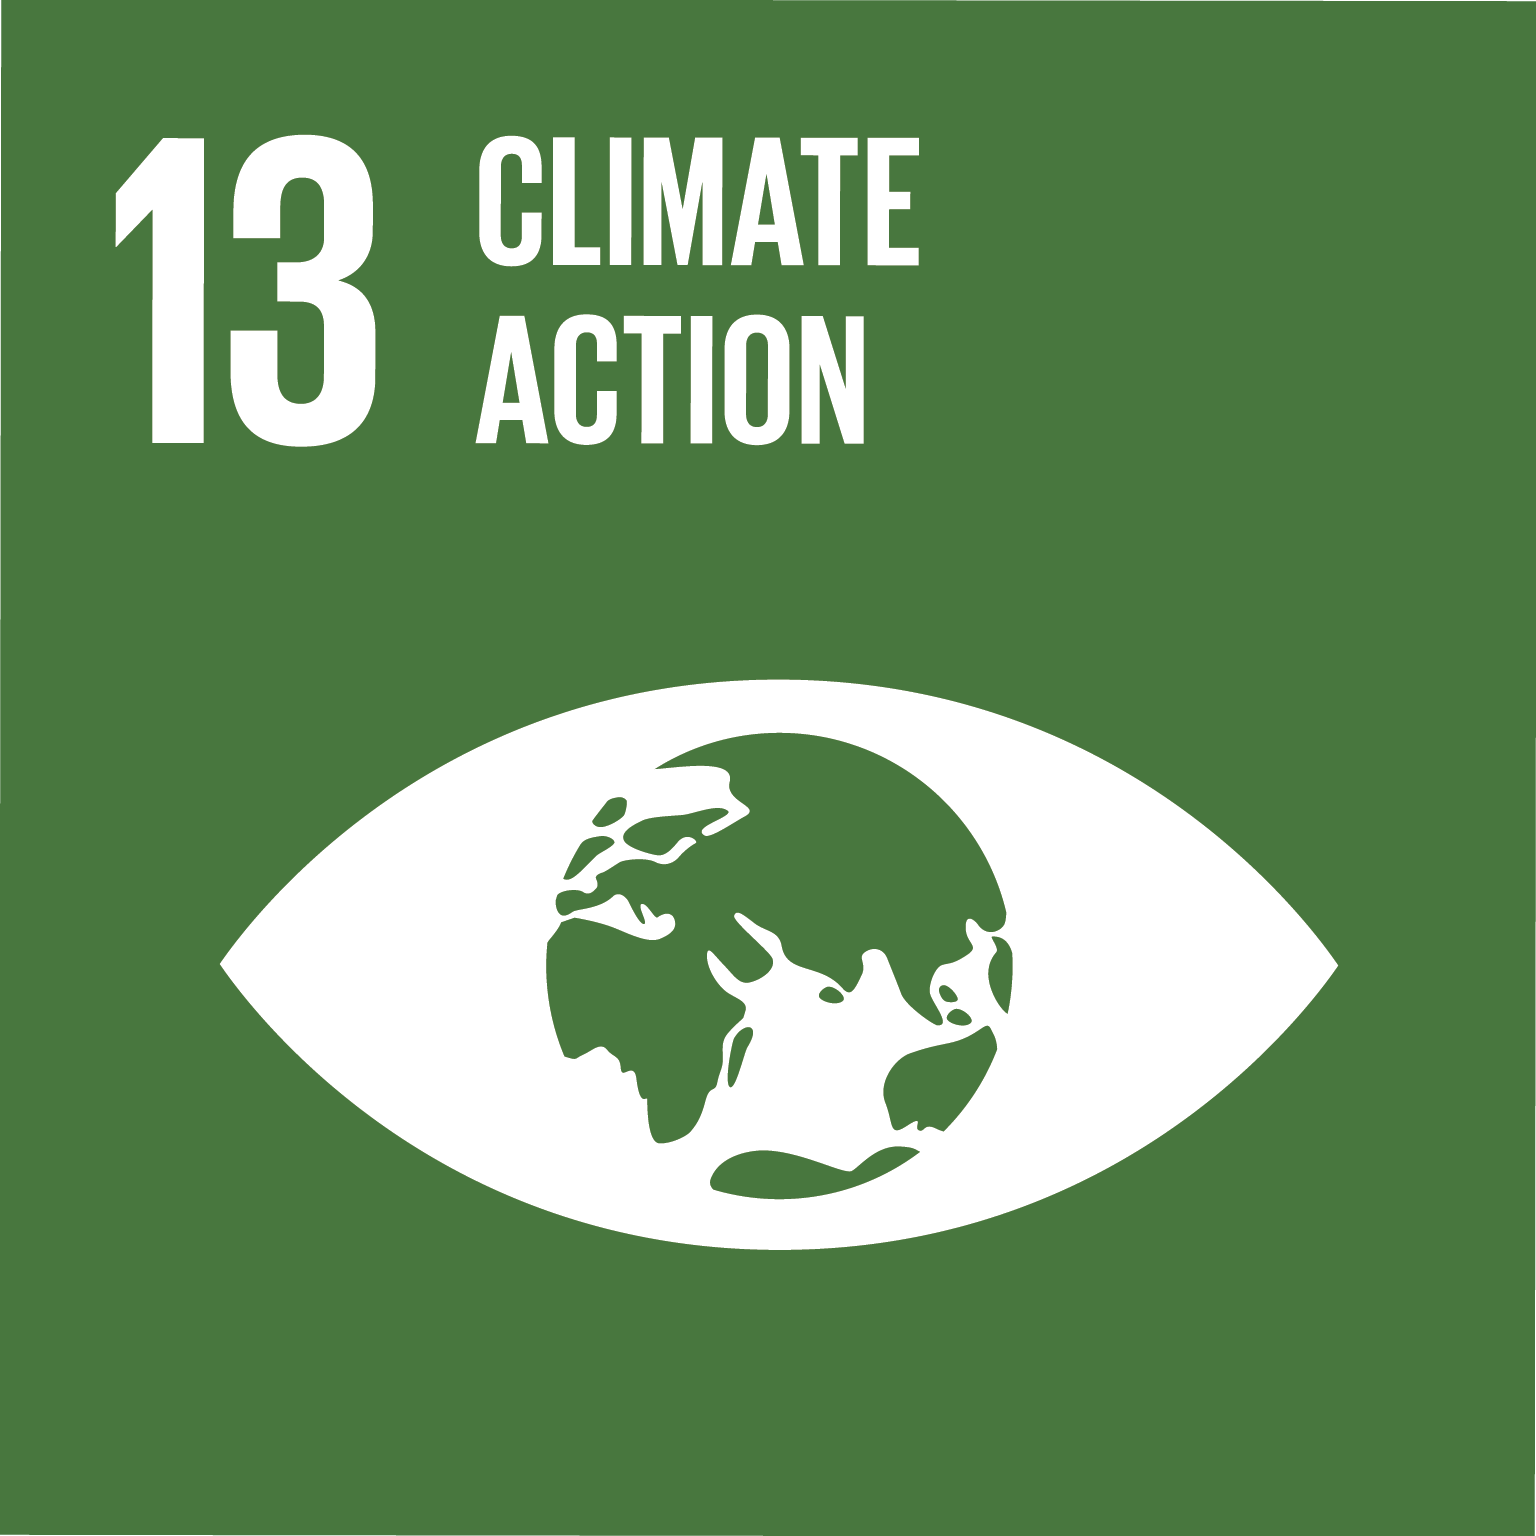
\includegraphics[height=4cm]{figures/sdg/sdg13.png}\hfill
    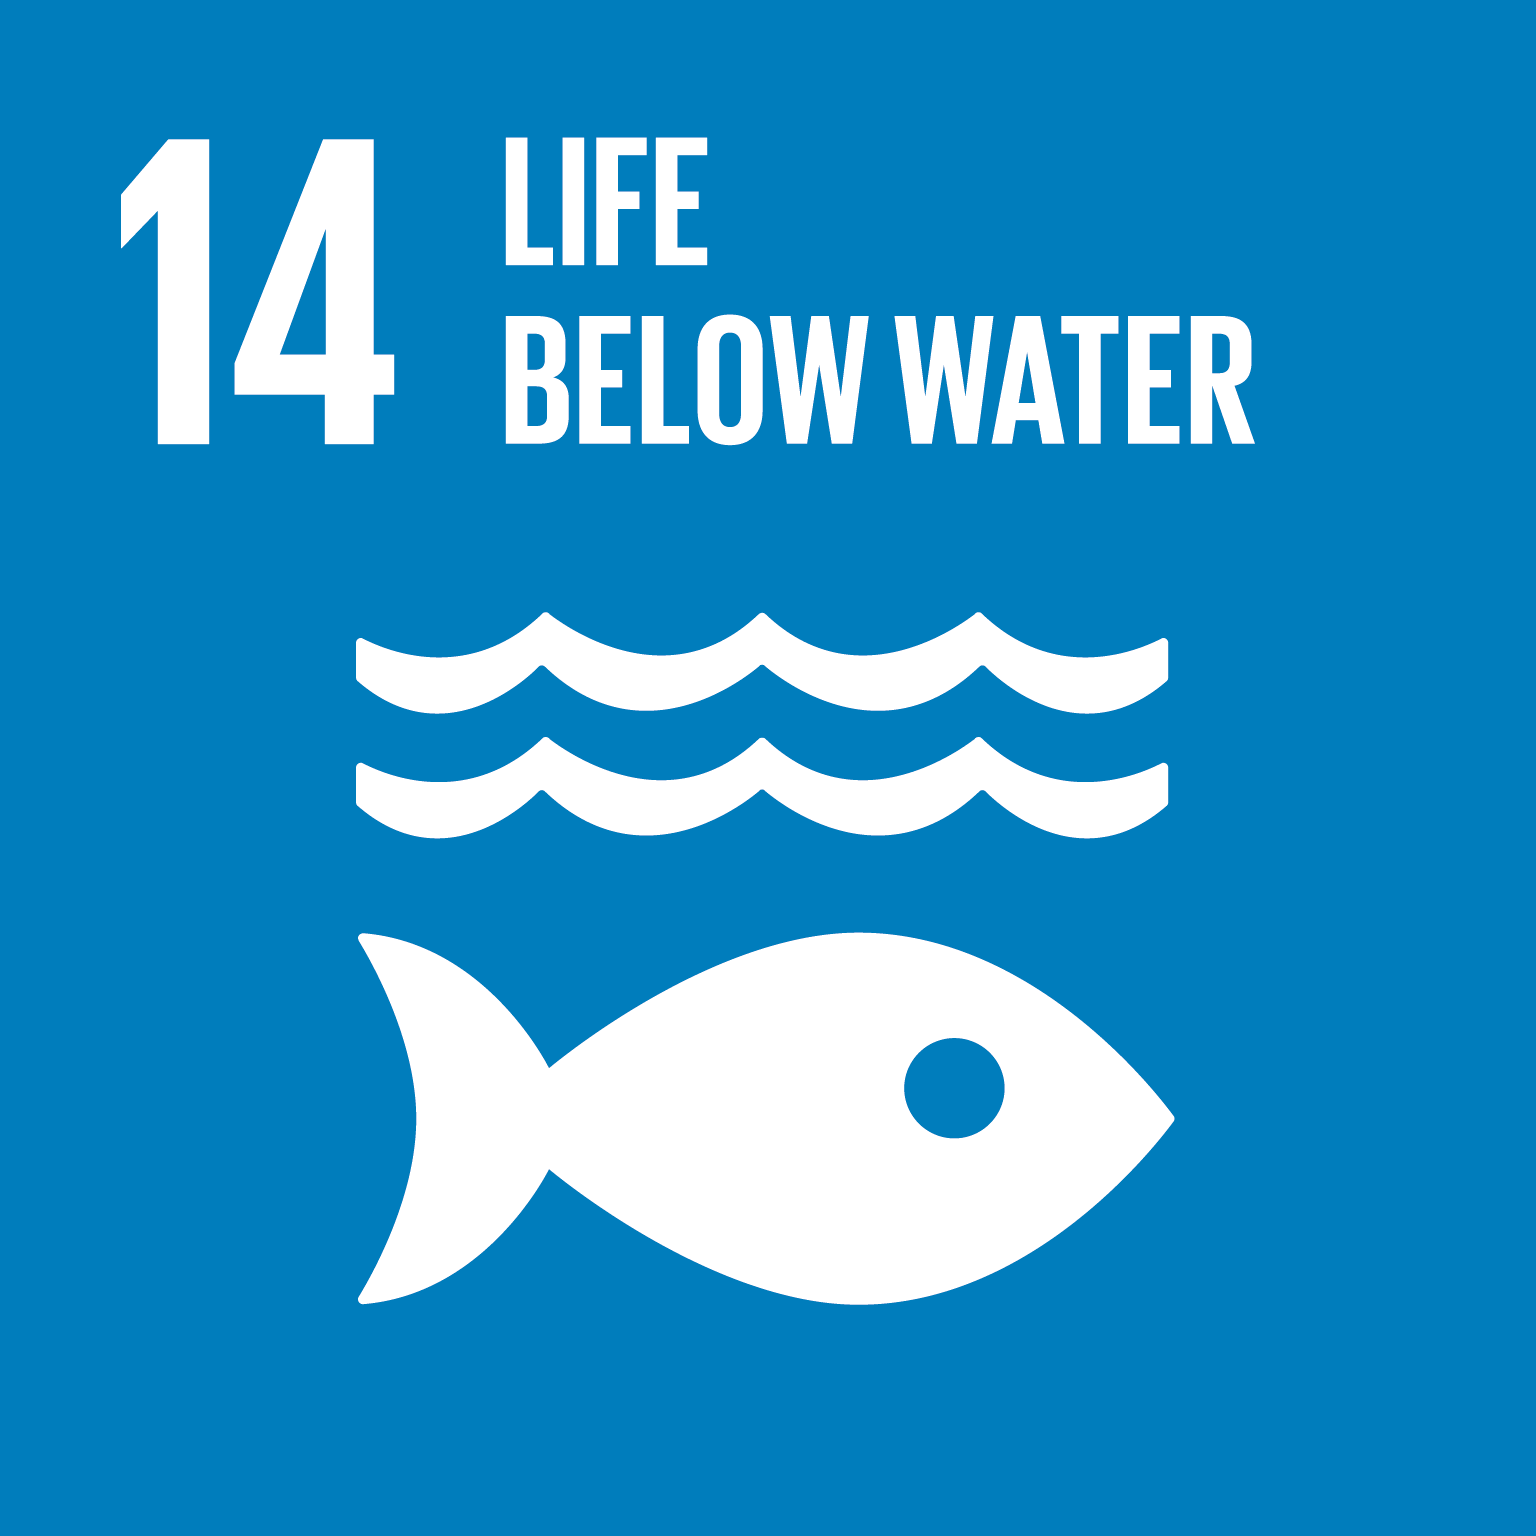
\includegraphics[height=4cm]{figures/sdg/sdg14.png}
    \caption[Sustainable Development Goals addressed by this thesis.]{\textbf{The
    three Sustainable Development Goals this thesis contributes to.} SDG~13
    (Climate Action), in particular target~13.3 on education, awareness and
    capacity; SDG~4 (Quality Education), on making complex knowledge accessible;
    and SDG~14 (Life Below Water), as the AMOC is part of the ocean system.
    Icons \textcopyright~United Nations. The content of this publication has not
    been approved by the United Nations and does not reflect its views.}
    \label{fig:sdg-alignment}
\end{figure}

% -------------------------------------------------------------------------
\section{Roadmap}
\label{sec:roadmap}

The thesis follows the detect--translate--evaluate arc in three parts. 

\textbf{Part~I --- DETECT} sets up the problem and the case: Chapter~\ref{ch:rqs} formalises the research questions, objectives and hypotheses; Chapter~\ref{ch:literature} reviews the relevant literature and locates the thesis within it; Chapter~\ref{ch:background} develops the physical and mathematical apparatus needed to treat the AMOC as an analysable object. 

\textbf{Part~II --- TRANSLATE} documents the constructive work: Chapter~\ref{ch:methodology} specifies the three-stage methodology; Chapter~\ref{ch:data_pipeline} presents the analytical pipeline that recovers the system's latent structure; Chapter~\ref{ch:translate} designs the representational conditions through which that structure is translated. 

\textbf{Part~III --- EVALUATE} closes the loop: Chapter~\ref{ch:userstudy} specifies the user study, Chapter~\ref{ch:results} reports its findings, Chapter~\ref{ch:discussion} interprets them, and Chapter~\ref{ch:conclusion} reflects on limitations, transferability and future work.
